% -*- root: cuthesis_masters.tex -*-
\section{Introduction}
\label{chap4:sec:introduction}
\setlength\parindent{24pt} 

In the development process, developers are constantly striving to maximize efficiency by delivering ever more sophisticated software by ever earlier deadlines. Pressure to meet projected release dates and output quotas raises the stakes and tempts many developers to consider options with long-term consequences which would otherwise be shelved on account of "creating more work in the future." \cite{kruchten2013technical} \cite{seaman2015technical}. Code smells such as god classes indicate faulty design principles and other factors that slow development and contribute to underlying technical debt \todo{ref}.Analysts have invoked the \emph{technical debt} metaphor time and again to draw parallels between the financial ramifications of assuming a loan, which will have to be repaid with interest, and the software development equivalent of writing code that temporarily serves the purpose or meets the deadline but incurs the effort of maintenance or repair at a later date \cite{cunningham1993wycash}. From the perspective of those who succumb to technical debt in handling time-sensitive deliveries, the looming expiration date of a temporary solution pales in comparison to the prospect of coming up empty-handed on the due date \cite{lim2012balancing}. In the end, technical debt is a last-ditch insurance policy against underperformance stemming from time constraints.




Predictably, as technical debt has become a more popular, if more stigmatized, recourse at developers' disposal, numerous advances have been made in detecting it, some metric-based and others comment-based. The former includes Marinescu's \cite{marinescu2004detection} methodology, which detects ``god class" code smells according to sets of rules and thresholds defined on various object-oriented metrics. The latter, advocated by Potdar and Shihab's \cite{ICSM_PotdarS14} methodology in recent work, flags recurring source code comment patterns that correlate with incidence of "self-admitted technical debt" (SATD). Moreover, the nature of the comments that developers leave has allowed occurrences of SATD to be subcategorized and analyzed accordingly.


Attitudes towards technical debt are beginning to shift, erring more on the side of caution, or even going so far as to assert that it is outright detrimental in terms of software maintenance and quality control \cite{zazworka2011investigating,spinola2013investigating,GuoSGCTSSS11,seaman2015technical,kruchten2013technical}. Empirical evidence, meanwhile, has not kept pace, yet without it developers will be misinformed as to the costs and benefits of technical debt and unequipped to decide responsibly whether it should be assumed in a given scenario, not to mention that they will lack effective strategies for keeping it in check once assumed.


Our work closes this gap as we study forty open-source projects that bring into focus the empirical links between both \SATD and god classes and software quality. Our inquiry pursues (i) whether god class and SATD-ridden files contribute more defects than files free of god classes and SATD, (ii) whether emerging defects can be traced to god and SATD changes and (iii) whether god- and SATD-related changes are associated with greater difficulty. As in the previous chapter, amount of churn, quantity of affected files and modified modules and change entropy all factor into the change difficulty calculation. We observed that: (i) no straightforward correlation exists between incidence of SATD, god files and incidence of defects, (ii) more future defects surfaced after performing god and SATD changes than non-god and non-SATD changes and (iii) god and SATD changes are more difficult to perform than non-god and non-SATD changes. Preliminarily, this concedes that the downsides of god classes and \SATD are increases in future defect density and change difficulty.


\section{Related Work}
\label{chap4:sec:related_work}

\subsection{Identifying and Detecting What Constitutes Code Smells}
Fowler and Beck \cite{fowler1999refactoring} originated the term "code smell" to designate various indicators of object-oriented design flaws which can undermine software maintenance. Code smells respond to the internal and external properties of the system elements they monitor. Though manual code smell detection warns developers of potential vulnerabilities, Marinescu \cite{Marinescu_ICETOOLS} observes that it is time-consuming, non-repeatable and non-scalable. Apart from this, the more familiar the software system is to a developer, the higher the risk of a subjective appraisal of its efficiencies and shortcomings, according to Mäntylä \cite{mantyla2003taxonomy} \cite{mantyla2004bad}, and one important corollary of this is that a developer's chances of overlooking design flaws increase. In order to surmount these drawbacks, Marinescu recommends enlisting code metrics to detect system volatilities, and in this spirit, several implementations of this departure from manual detection have been devised \cite{marinescu2004detection} \cite{Marinescu_PhD} \cite{Marinescu_IBM_JRD} \cite{lanza2007object}.

\section{Approach}
\label{chap4:sec:approach}
As we persevere in studying the interplay between \SATD, god classes and software quality, the latter must be made amenable to objective quantification \cite{Kamei-tse-2013,Kim-tse-2008,sliwerski-msr-2005}. The precedent in accomplishing this task has been to count the defects in SATD files and calculate the rate of future defect introduction among SATD changes, expressed as a percentage. Deferring to the technical debt metaphor and its concept of accruing "interest" to be paid in the long run, we also measure software quality in terms of SATD change difficulty, which we calculate as stipulated earlier. With these metrics standardized, we entertain the research questions that follow:

\begin{itemize}
	\vspace{0.2cm}
	\item {\bf RQ1:} Do god files have more defects than non-god files?\\
	%\vspace{0.2cm}
	\item {\bf RQ2:} Do god-related changes introduce future defects?\\
	%\vspace{0.2cm}
	\item {\bf RQ3:} Are god-related changes more difficult than non-god changes?
	%\vspace{0.2cm}
\end{itemize}

We devised a suitable method of operation, visualized in Figure \ref{fig:CH4_Process_overview}, in order to guide our inquiry into these questions. We initiated the process by mining the source code repositories and pulling source code files on a project-by-project basis (steps 1-2). Afterwards the source code files were parsed and comments extracted (step 3). We then implemented Potdar and Shihab's proposed source code comment patterns to identify all instances of SATD, counted defects file-wide, and isolated defect-inducing changes by means of the SZZ algorithm (steps 4-5).

\begin{figure}[t]
	\centering
	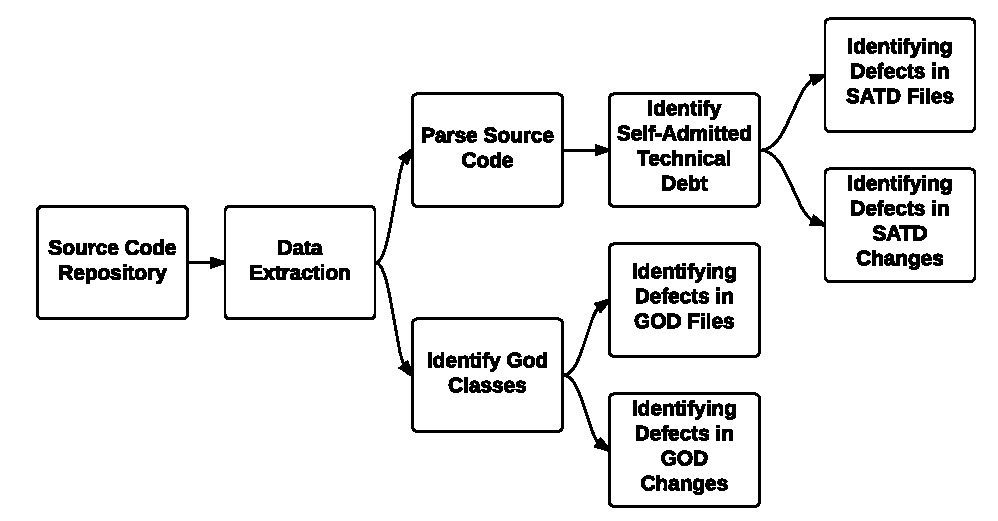
\includegraphics[width=150mm]{figures/chapter4/approach}
	\caption{Approach overview.}
	\label{fig:CH4_Process_overview}
\end{figure}


\subsection{Data Extraction}

Drawing on forty open-source software projects, we attempted to randomize our sample by domain and size while verifying that each project had amassed substantial source code comments from a wide array of contributors, which Potdar and Shihab's SATD detection technique presupposes. Projects "just getting off the ground" in terms of their development history were omitted, and all projects selected were available to software development researchers.


Given the extent to which our approach to locating \SATD relies on source code comments, we downloaded the most recent versions of the relevant systems, filtered this input to generate source code, and excluded all files lacking source code comments (\eg{} CSS, XML, JSON). As for comments suspected of indicating no SATD, e.g. license comments, commented source code, Javadoc comments, etc., four filtering heuristics were deployed to remove them from the results.


Tables \ref{table:ch4_projects_statistics} and \ref{table:ch4_projects_statistics_2} showcase some key identifiers and statistics for each project, including (i) which release was downloaded, (ii) the number of lines of code it contains, (iii) the number of comment lines, (iv) a source code file count, (v) the number of committers in the project's development history and (vi) its commit count.

\begin{landscape}


\begin{table}[htbp]
	\small
	\centering
	\caption{Characteristics of the studied projects.}
	\begin{adjustbox}{width=1.3\textwidth}


		\begin{tabular}{l|l|c|c|c|c|c}
			\hline
			\textbf{Project}           & \textbf{Release} & \textbf{\# Lines of Code} & \textbf{\# Comment Lines} & \textbf{\# Files} & \textbf{\# Committers} & \textbf{\# Commits} \\ \hline
			\textbf{Apache OpenNLP}    & 1.7.1            &          163,114           &           30,581           &        861        &           11           &        1,339         \\ \hline
			\textbf{Apache Camel}      & 2.18.0           &          1,626,040          &          430,818           &       17,046       &          333           &        25,461        \\ \hline
			\textbf{Apache Habse}      & ‎1.2.4           &          1,310,985          &          251,409           &       3,243        &          166           &        12,531        \\ \hline
			\textbf{Apache Groovy}     & 2.4.2            &          286,920           &           85,885           &       1,517        &          262           &        13,422        \\ \hline
			\textbf{Apache Oltu}       & 1.0.2            &           267,88           &           7,386            &        300        &           14            &         842         \\ \hline
			\textbf{Apache Maven}      & 3.3.9            &          150,724           &           34,830           &       1,540        &           81           &        10,370        \\ \hline
			\textbf{Apache Karaf}      & 5.4.0            &          155,675           &           32,906           &       1,467        &           86           &        5,666         \\ \hline
			\textbf{Apache Hama}       & 0.6.4            &           855,64           &           22,545           &        499        &           22           &        1,592         \\ \hline
			\textbf{Apache Tomee}      & 1.7.4            &          854,611           &          212,542           &       6,297        &           35           &        10,257        \\ \hline
			\textbf{Apache Deltaspike} & 1.7.2            &          149,871           &           45,722           &       1,842        &           48           &        2,044         \\ \hline
			\textbf{Apache Curator}    & 2.10.0           &          124,077           &           18,458           &        525        &           66           &        1,813         \\ \hline
			\textbf{Apache Calcite}    & 1.10.0           &          448,820           &          110,410           &       1,702        &          102           &        2,180         \\ \hline
			\textbf{Apache Poi}        & 3.15             &          644,284           &          182,823           &       3,298        &           39           &        7,963         \\ \hline
			\textbf{Apache Zeppelin}   & 0.6.2            &          124,865           &           15,314           &        552        &          201           &        2,642         \\ \hline
			\textbf{Apache Ant}        & 1.9.7            &          343,010           &          109,150           &       1,927        &           62           &        13,425        \\ \hline
			\textbf{Apache Stanbol}    & 1.0.0            &          339,699           &          107,208           &       2,044        &           25           &        3,398         \\ \hline
			\textbf{Apache Kafka}      & 0.10.1           &          152,685           &           33,368           &       1,002        &          300           &        2,734         \\ \hline
			\textbf{Apache Tika}       & 1.13             &          142,786           &           38,984           &        992        &           54           &        3,209         \\ \hline
			\textbf{Apache Felix}      & ‎5.4.0           &          837,955           &          211,404           &       5,039        &           51           &        13,240        \\ \hline
			\textbf{Apache Phoenix}    & 4.9.0            &          396,054           &           69,326           &       1,620        &           59           &        1,748         \\ \hline
		\end{tabular}
		\label{table:ch4_projects_statistics}

\end{adjustbox}

\end{table}

\end{landscape}



\begin{landscape}

	
	
	\begin{table}[htbp]
		\small
		\centering
		\caption{Characteristics of the studied projects.}
		\begin{adjustbox}{width=1.3\textwidth}
			
			
			\begin{tabular}{l|l|c|c|c|c|c}
				\hline
				\textbf{Project}           & \textbf{Release} & \textbf{\# Lines of Code} & \textbf{\# Comment Lines} & \textbf{\# Files} & \textbf{\# Committers} & \textbf{\# Commits} \\ \hline
				\textbf{Apache Wicket}     & 7.5.9            & 548,923                    &          191,279           &       4,830        &           80           &        19,574        \\ \hline
				\textbf{Apache Aurora}     & 0.16.0           & 317,551                    &           70,774           &       1,284        &          105           &        3,639         \\ \hline
				\textbf{Apache Ignite}     & 1.6              & 1,498,260                   &          443,157           &       7,361        &          117           &        17,933        \\ \hline
				\textbf{Apache Helix}      & 0.7.1            & 141,632                    &           34,430           &        900        &           32           &        2,266         \\ \hline
				\textbf{Apache Archiva}    & 2.2.1            & 191,743                    &           33,641           &       1,172        &           41           &        7,742         \\ \hline
				\textbf{Apache Struts}     & 2.5              & 316,495                    &           83,911           &       2,307        &           65           &        4,634         \\ \hline
				\textbf{Apache Derby}      & 10.13.1.1        & 1,271,629                   &          386,703           &       3,023        &           37           &        8,127         \\ \hline
				\textbf{Apache Ambari}     & ‎2.4.2           & 2,220,418                   &          421,937           &       10,223       &          119           &        18,025        \\ \hline
				\textbf{Apache Nifi}       & 1.0.0            & 576,512                    &          118,806           &       3,493        &          120           &        2,826         \\ \hline
				\textbf{Apache Tiles}      & 3.0.7            & 51,487                     &           20,173           &        599        &           16           &        1,455         \\ \hline
				\textbf{Apache Shiro}      & ‎1.3.2           & 81,131                     &           36,854           &        727        &           22           &        1,641         \\ \hline
				\textbf{Apache Usergrid}   & 2.1.0            & 605,286                    &          114,999           &       2,619        &          110           &        10,621        \\ \hline
				\textbf{Apache Nutch}      & 2.3              & 104,214                    &           27,478           &        843        &           37           &        2,217         \\ \hline
				\textbf{Apache Zookeeper}  & 3.4.9            & 196,008                    &           38,867           &        814        &           21           &        1,468         \\ \hline
				\textbf{Apache Mina}       & 2.0.16           & 45,588                     &           14,336           &        340        &           29           &        2,400         \\ \hline
				\textbf{Apache Cxf}        & 3.1.8            & 988,585                    &          196,520           &       8,806        &           81           &        12,302        \\ \hline
				\textbf{Apache CloudStack} & 4.9.0            & 1,423,346                   &          207,036           &       6,424        &          412           &        29,931        \\ \hline
				\textbf{Apache Oozie}      & 4.3.0RC0         & 256,423                    &           49,510           &       1,239        &           22           &        1,772         \\ \hline
				\textbf{Apache Kylin}      & 1.5.4.1          & 217,645                    &           45,320           &       1,227        &           89           &        5,121         \\ \hline
				\textbf{Apache Flink}      & 1.1.2            & 791,670                    &          195,738           &       4,154        &          325           &        9,513         \\ \hline
			\end{tabular}
			\label{table:ch4_projects_statistics_2}
			
		\end{adjustbox}
		
	\end{table}
	
\end{landscape}


\subsection{Scanning Code and Extracting Comments}

Having isolated the source code from all of the projects under investigation, we tasked a Python-based tool with extracting the source code comments. Beyond this, the tool reveals each comment's type (i.e. single-line or block comments), the name of its host file, and its line number. The Count Lines of Code (CLOC) tool ~\cite{cloc} double-checks the Python-based tool, and provided that there is no discrepancy between the total number of lines of comments both yield, we have confidence in the accuracy of the tool we developed.

\subsection{Filter Comments}


The content of source code comments is as loosely determined as the formalities that developers observe in making them. Depending on what it is the commenter wishes to call attention to or notify future contributors of, the comments might situate the project within the circumstances of its development, make recommendations for revising the code at a later date, acknowledge who wrote which pieces or who made which fixes, or confide that self-admitted technical debt has been assumed. Efforts should be made to decrease the volume of comments, especially when sifting through them in search of \SATD confessions. For this reason, we make use of several filtering heuristics to focus our search query.\par

A Python-based tool reads data retrieved from parsed source code, initiates the filtering heuristics and stores the results in the database. The retrieved data specify each class or comment's starting and ending line numbers as well as Java syntax comment type (i.e., Single-line, Block or Javadoc). Once this information is acquired, the filtering heuristics are processed. \par

Self-admitted technical debt is seldom indicated in comments left prior to class declaration, e.g. license comments, among others, so we benefit from any mechanism that identifies and omits such distractors without also omitting comments that incorporate Java IDE task annotations (i.e. "TODO:", "FIXME:" or "XXX:"). If a comment features any of these keywords, tasks related to the comment will be added to an IDE-generated list for ease of access. As for separating pre- and post-class declaration comments, the number of the line in which class is declared marks the crucial cutoff in that any preceding comments are targeted for removal.\par

Comment type matters insofar as cumbersome comments stitched together from single-line comment components (and not block comments) impede message interpretation for comments read one by one. A heuristic that pinpoints and collapses sequences of adjacent single-line comments into block comments overcomes the comment type issue.\par



Commented source code does not indicate \SATD in our experience, but rather either code not used at all or code used exclusively for debugging. To eliminate this distractor, we use a regular expression to remove typical Java code structures, i.e. public, private, for, exception, etc.\par


Most IDEs auto-generate comments when creating a method, constructor, try catch, etc. Due to the nature of the auto-generation of these comments, the likelihood of them containing SATD is nonexistent. The majority of Javadoc comments also fail to mention SATD, and those that do are annotated with at least one task (i.e. "TODO:", "FIXME:", "XXX:"). This criterion allows our heuristic to determine which Javadoc comments should be salvaged versus ignored, while no distinction is necessary for auto-generated comments. We designed a regular expression to apply the criterion by checking for task annotations before omitting the comment.\par




The procedure was conceived with the intention of factoring out the contribution of noise, which ultimately improves the quality of the comment dataset by reducing cases of SATD false positives and facilitating the most applicable comments.\par



\subsection{Identifying Self-Admitted Technical Debt}
\label{ch4_td}


Our analysis hinges on locating \SATD at two levels: (i) file level and (ii) change level.

\noindent\textbf{SATD files:}
We emulated Potdar and Shihab \cite{ICSM_PotdarS14} in identifying SATD on the basis of 62 different templates recurring in multiple projects at various frequencies. If a comment is found to match one or more of these templates, among them \textit{"hack, fixme, is problematic, this isn't very solid, probably a bug, hope everything will work, fix this crap"}, it is taken to mean that SATD is present to some degree. The remaining patterns we designated for use in this inquiry are accessible online \footnote{http://users.encs.concordia.ca/\textasciitilde
eshihab/data/ICSME2014/data.zip}.


We subsequently abstract up from individual comment patterns in order to assign each file its proper label. {\em SATD files} are those that have SATD comments and are thus the ones we contemplate in addressing RQ1, whereas {\em non-SATD files} do not have comments matching any of the 62 tell-tale patterns nor do they concern us here.\\


\noindent\textbf{SATD changes:}
At the change level, all the files touched by the same change are scrutinized for evidence of \SATD. If any one of them is determined to be an SATD file, the whole change is classified as an SATD change. Alternatively, if none of the files touched by a change is an SATD file, the whole change falls into the non-SATD change category. SATD comments are shown to account for less than 6.10\% and SATD files for somewhere between 1.37 and 25.03\% of the respective totals for all systems in Table~\ref{table:projects_satd_god_percentage} and \ref{table:projects_satd_god_percentage2}, where each system's proportions are listed separately for comparison.

\begin{landscape}
	
	
	\begin{table}[htbp]
		\small
		\centering
		\caption{Percentage of SATD and god of the analyzed projects.}
		\begin{adjustbox}{width=1.0\textwidth}
			
			
			\begin{tabular}{l|c|c|c}
				\hline
				\textbf{Project}  & \textbf{SATD Comments (\%)}  & \textbf{SATD Files (\%)} & \textbf{God Files (\%)} \\ \hline
				\textbf{Apache OpenNLP} &  2.66 & 19.02 & 14.77   \\ \hline
				\textbf{Apache Camel} &  0.95 & 3.53 & 12.95    \\ \hline
				\textbf{Apache Habse} & 1.69 &  18.29 & 15.05    \\ \hline
				\textbf{Apache Groovy} &  3.41 & 13.67 & 14.52    \\ \hline
				\textbf{Apache Oltu} &  1.91 & 5.67 & 14.27    \\ \hline
				\textbf{Apache Maven} &  3.76 & 10.65 & 13.92    \\ \hline
				\textbf{Apache Karaf} &  2.40 & 7.44 & 14.58   \\ \hline
				\textbf{Apache Hama} &  1.44 & 11.24 & 14.48    \\ \hline
				\textbf{Apache Tomee} &  1.94 & 7.16 & 14.33   \\ \hline
				\textbf{Apache Deltaspike} &  3.95 & 9.28 & 9.26    \\ \hline
				\textbf{Apache Curator} &  0.99 & 5.34 & 15.32    \\ \hline
				\textbf{Apache Calcite} &  1.67 & 12.97 & 14.54    \\ \hline
				\textbf{Apache Poi} &  2.11 & 16.79 & 14.43    \\ \hline
				\textbf{Apache Zeppelin} &  1.62 & 9.37 & 14.87    \\ \hline
				\textbf{Apache Ant} &  2.23 & 20.56 & 14.60   \\ \hline
				\textbf{Apache Stanbol} &  4.03 & 25.03 & 14.06   \\ \hline
				\textbf{Apache Kafka} &  1.56 & 7.73 & 11.71    \\ \hline
				\textbf{Apache Tika} &  3.29 & 19.28 & 14.40    \\ \hline
				\textbf{Apache Felix} & 1.88 & 9.72 & 13.59   \\ \hline
				\textbf{Apache Phoenix} &  3.34 & 13.81 & 13.47    \\ \hline
				
			\end{tabular}
			\label{table:projects_satd_god_percentage}
			
		\end{adjustbox}
		
	\end{table}
	
\end{landscape}



\begin{landscape}
	
	
	
	\begin{table}[htbp]
		\small
		\centering
		\caption{Percentage of SATD and god of the analyzed projects.}
		\begin{adjustbox}{width=1.0\textwidth}
			
			
			\begin{tabular}{l|c|c|c}
				\hline
				\textbf{Project}  & \textbf{SATD Comments (\%)}  & \textbf{SATD Files (\%)} & \textbf{God Files (\%)} \\ \hline
				\textbf{Apache Wicket} &  0.89 & 5.29 & 11.52    \\ \hline
				\textbf{Apache Aurora} &  3.97 & 14.27 & 14.91    \\ \hline
				\textbf{Apache Ignite} &  0.26 & 3.12 & 13.50   \\ \hline
				\textbf{Apache Helix} &  4.02 & 18.09 & 15.62    \\ \hline
				\textbf{Apache Archiva} &  6.05 & 17.71 & 12.61    \\ \hline
				\textbf{Apache Struts} &  1.85 & 8.07 & 12.39    \\ \hline
				\textbf{Apache Derby} &  1.20 & 22.66 & 14.37    \\ \hline
				\textbf{Apache Ambari} &  2.29 & 8.76 & 13.31   \\ \hline
				\textbf{Apache Nifi} &  0.87 & 4.62 & 13.29    \\ \hline
				\textbf{Apache Tiles} &  0.17 & 1.37 & 10.90    \\ \hline
				\textbf{Apache Shiro} &  2.67 & 15.86 & 12.85    \\ \hline
				\textbf{Apache Usergrid} &  2.20 & 11.20 & 12.33    \\ \hline
				\textbf{Apache Nutch} &  2.17 & 12.25 & 15.60    \\ \hline
				\textbf{Apache Zookeeper} &  1.71 & 10.31 & 13.82   \\ \hline
				\textbf{Apache Mina} &  1.12 & 5.99 & 14.71   \\ \hline
				\textbf{Apache Cxf} &  2.78 & 6.87 & 14.04   \\ \hline
				\textbf{Apache CloudStack} &  1.98 & 10.42 & 14.04   \\ \hline
				\textbf{Apache Oozie} &  1.63 & 9.73 & 15.81   \\ \hline
				\textbf{Apache Kylin} &  1.64 & 8.06 & 15.38   \\ \hline
				\textbf{Apache Flink} &  0.57 & 3.72 & 14.84   \\ \hline
				
			\end{tabular}
			\label{table:projects_satd_god_percentage2}
			
		\end{adjustbox}
		
	\end{table}
	
\end{landscape}

\subsection{God Class}
God classes are classes that consolidate trivial class workloads and avoid task delegation for all but the simplest of operations and are distinguishable on account of their high complexity, low inner-class cohesion and frequent foreign class data access \cite{lanza2007object}. Object-oriented design advocates a one-to-one correspondence between classes and responsibilities, which god classes violate by definition \cite{lanza2007object}. Due to their size and the extent to which they are tied to other classes, god classes can make it more difficult to understand the system \cite{fowler1999refactoring} and are expected to be more susceptible to defects during system maintenance. The higher the incidence of defects, the more often changes will have to be performed and the bigger those changes will be, compounding maintenance over time \cite{fowler1999refactoring} \cite{lanza2007object}.

\subsection{Identifying God Classes}
\label{ch4_god}

To perform our analysis, we need to identify god classes at two levels: (i) file level and (ii) change level.

\noindent\textbf{god files:} To identify god classes, we followed the methodology outlined by Marinescu \cite{marinescu2004detection}, who proposed an approach to specify and detect
code smells, specifically ``god classes'', based on metric-based heuristics where god classes are identified according to sets of rules and thresholds defined on various object-oriented metrics. The formula provided below \ref{equation:1} operates on three metrics, namely, weighted method count (WMC), tight class cohesion (TCC) and access to foreign data (ATFD), and generates one of two outputs. If the output is 1, then the class to which the formula is applied is a god class; if 0, it is a non-god class.

\noindent\textbf{god changes:}
To study the impact of god classes at the change level, we must first identify which classes are god classes and which are non-god classes. By analogy with the technique used to identify SATD and non-SATD changes, we consider any change containing at least one god file to be a god change and those containing no god files to be non-god changes. 


\begin{figure}[h]
\[GodClass(C) = \left\{\begin{matrix}
1& (AFTD(C), HigherThan(1))  \wedge ((WMC(C), TopValues(25\%)) \vee \\ 
 & (TCC, BottomValues(25\%)))\\ 
0& else
\end{matrix}\right.\]
\caption{God Class Detection Equation}
\label{equation:1}
\end{figure}

The equation in Figure~\ref{equation:1} above describes how we detect a god class, where 


\begin{itemize}
\item[$\bullet$] \textbf{Weighted Method Count (WMC)} is the sum of the statistical complexity of all methods in a class \cite{Chidamber_Kemerer_94}. McCabe’s cyclomatic complexity \cite{McCabe_1976} is used as a complexity measure for all class methods.
\item[$\bullet$] \textbf{Tight Class Cohesion (TCC)} is the number of directly connected public methods in a class \cite{Bieman:1995:CRO:223427.211856}.
\item[$\bullet$] \textbf{Access to Foreign Data (ATFD)} is the number of external classes whose attributes are accessed either directly or indirectly (by accessor methods) \cite{Marinescu_PhD}
\end{itemize}

\subsection{Identifying Defects in SATD Files and SATD Changes}
\label{ch4_bugs_td}

According to Sliwersky \textit{et al.} \cite{sliwerski-msr-2005}, expressions denoting defect identifiers, e.g. "fixed issue", ``bug ID", ``fix", ``defect", ``patch", ``crash", ``freeze", ``breaks", ``wrong", ``glitch", ``properly", and ``proper", ordinarily certify that an earlier mistake has been corrected when recorded in control system change logs. Other work has proposed comparable methodologies for tracking fault-inducing changes until repaired \cite{Kamei-tse-2013, Kim-tse-2008, sliwerski-msr-2005}. Next we pull each defect report from its corresponding issue tracking system, i.e. Bugzilla \footnote{https://www.bugzilla.org} or JIRA \footnote{https://www.atlassian.com/software/jira}, and comb for all pertinent details.


Once the SATD files and SATD changes have been separated, we go about determining the number of file defects and identifying any defect-inducing changes in the same way foregoing research has ~\cite{Kamei-tse-2013, Kim-tse-2008, sliwerski-msr-2005}.

\noindent\textbf{Defects in files:}
A file defect count is a prerequisite to any defectiveness comparison between SATD and non-SATD files. With this in mind, we first view a file's history and extract all the changes that have touched it. The list this produces is then shortened as change log searches return only results consistent with keywords indicating corrective changes. Among these keywords we have: ``fixed issue \#ID'', ``bug ID'',  ``fix'',  ``defect'',  ``patch'', ``crash'',  ``freeze'', ``breaks'', ``wrong'', ``glitch'' and ``proper''. We refer to the defect report in the event of a defect identification in order to be certain that the defect is attributable to a system under investigation. This extra step must be undertaken because in communities like Apache, one issue tracking system serves several products.  At this point, issue IDs in the change logs that turn out to be false positives are discarded and the true positives point out the defect-fixing changes, i.e. we take the number of defects in a file to be equal to the number of corrective changes.

\noindent \textbf{Defect-inducing changes:}
Along the same lines, we search the commit messages using regular expressions that convey defect fixes as a means of establishing whether a given change is corrective. Particularly, we search the change logs for keywords such as: ``fixed issue \#ID'', ``bug ID'',  ``fix'',  ``defect'',  ``patch'', ``crash'',  ``freeze'', ``breaks'', ``wrong'', ``glitch'', and ``proper''. Likewise, defect identification numbers can clarify which defects the changes have in fact repaired.\\

After the corrective changes have been obtained, we find all prior changes that have touched the code utilizing the \texttt{blame} command. Our criterion for identifying the change that induced the defect is that it must be closest to yet still in advance of the defect report date such that it was the last change made before the defect emerged. In the absence of a defect report, we execute the SZZ~\cite{sliwerski-msr-2005} or approximate (ASZZ) algorithm~\cite{Kamei-tse-2013} and hold the last change before the corrective change to have induced the defect, as has been done in earlier work~\cite{Kamei-tse-2013}. This algorithm currently represents the standard all alternative methods of identifying defect-inducing changes are weighed against.

\section{Case Study Results}
\label{chap4:sec:case_study_results}

\begin{figure}[tb]
	\centering
	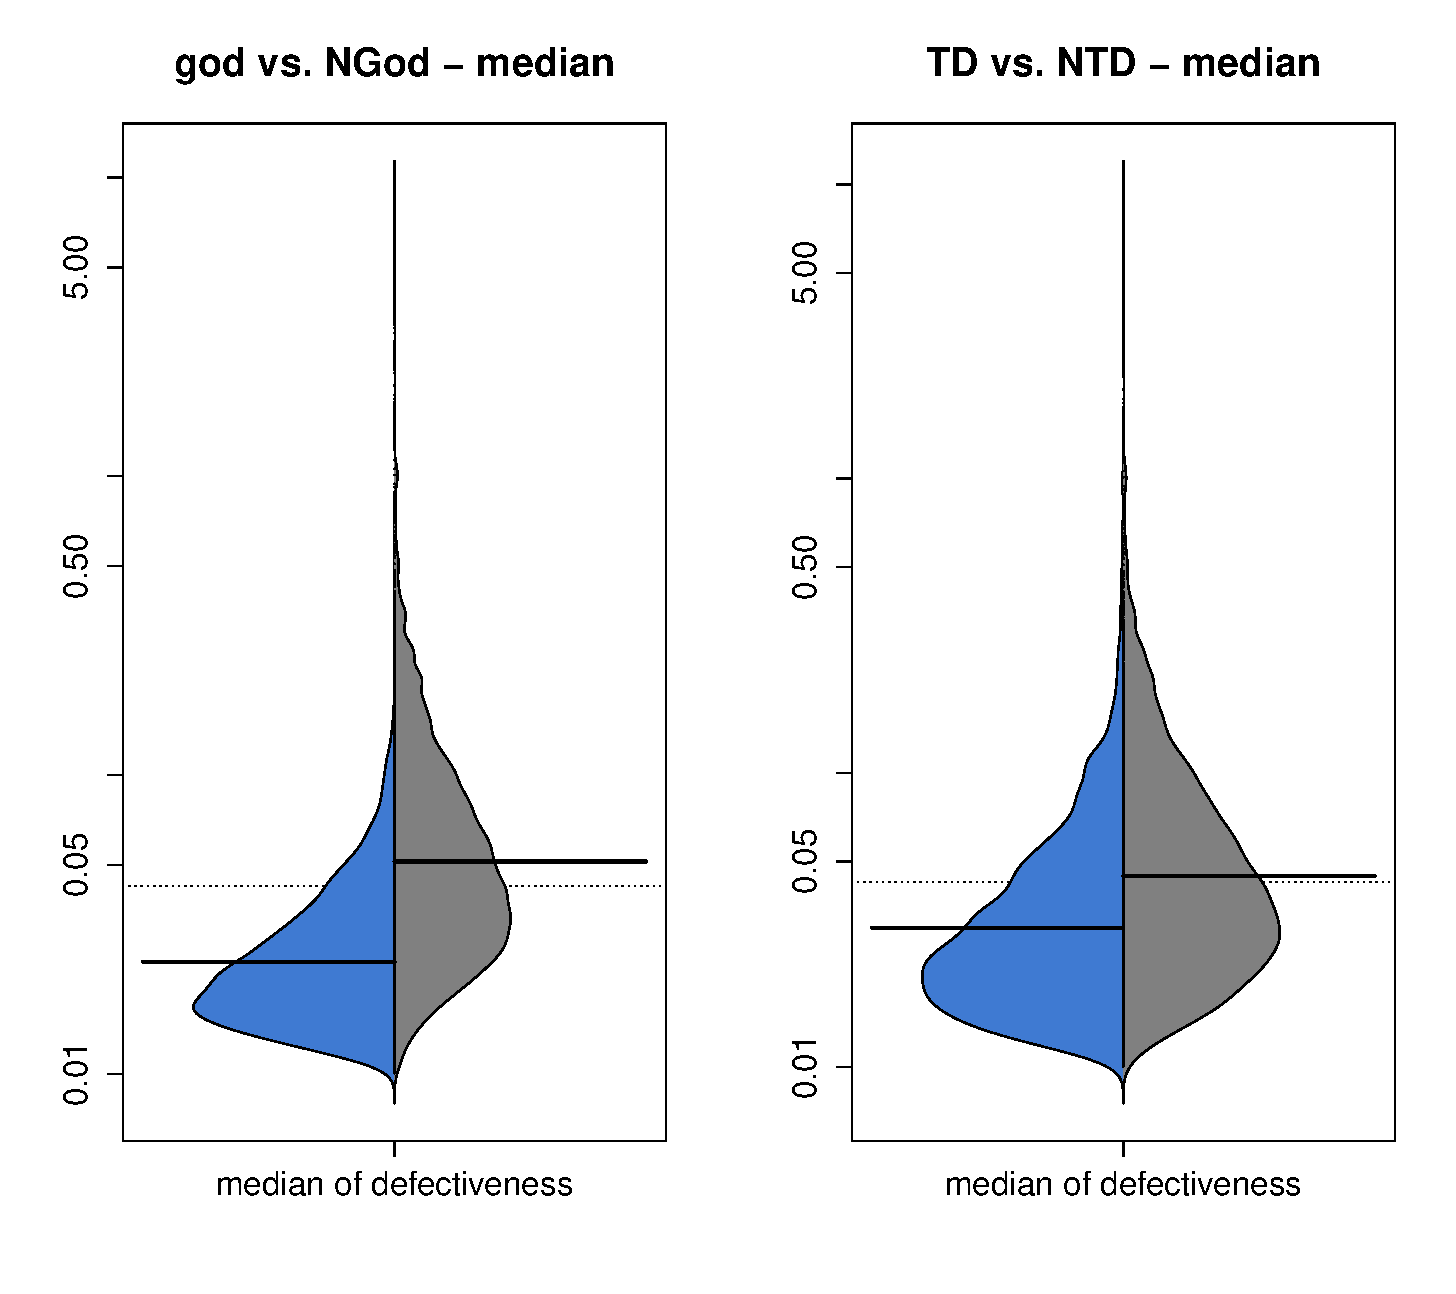
\includegraphics[width=140mm]{figures/chapter4/rq1_defectivness_distrubution}
	\caption{Percentage of defect fixing changes for SATD and NSATD files.}
	\label{figure:ch4_number_of_fixing_changes_TD_vs_NTD}
\end{figure}

In this section, we present the empirical outcomes of our inquiry into the correlation between self-admitted technical debt, god classes and software quality. Statistics and results are listed for all individual projects, accompanied by cross-project comparisons.

Each of the three research questions is restated below, where we summarize its motivation, our approach in treating it, and the conclusions we reached as a result.

\sultan{stopped here}
\subsection*{\chapterIVrqI}


\noindent{\textbf{Motivation:}}
Reluctance to resort to code smells and technical debt suggests that most developers believe these adversely affect software quality, and what research has been conducted supports this conviction~\cite{zazworka2011investigating}. \sultan{I'm not sure how to incorporate god classes in this case since there has been a lot of work that studied their impact on software quality} The potential drawbacks of SATD, meanwhile, have remained unexplored despite its research-affirmed ubiquity in software projects \cite{ICSM_PotdarS14}.

Researchers and developers should be better equipped to negotiate the long-term risks of SATD and have empirical evidence in hand that identifies concrete issues its use can bring about and raises SATD literacy within the community at large.


\noindent{\textbf{Approach:}}
We compare god files versus non-god files and SATD files versus non-SATD files in terms of defect-proneness as we take up RQ1.


\noindent\textbf{Comparing god and non-god files:}
The God Class Detection Equation proposed by \cite{marinescu2004detection} provides a way to identify god classes using object-oriented metrics. Files are fed to the equation and depending on the output are labeled either god or non-god files. We calculate the percentage of defect-fixing changes for each file in both categories based on $\frac{\left (\frac{\#~of~fixing~changes}{total~\#~changes} \right )}{SLOC}$. We normalize our data since files can have different amounts of changes and apply a test designed to measure whether the differences between the categories are statistically significant.

The Mann-Whitney~\cite{mann1947test} test accomplishes this non-parametrically and is thus capable of handling non-normal distributions (of which our data's distribution is one example), unlike parametric alternatives. A statistically significant difference returns a p-value of at most 0.05 ($p <= 0.05$).


\noindent\textbf{Comparing SATD and non-SATD files:}
We identify SATD files in accordance with the procedure detailed in Section~\ref{td} in the process, labeling files containing any number of SATD comments as SATD files and all others non-SATD files. These two file categories (SATD and non-SATD) undergo calculations yielding the percentage of defect-fixing changes, we calculate that based on $\frac{\left (\frac{\#~of~fixing~changes}{total~\#~changes} \right )}{SLOC}$ , which, unlike pure counts, standardizes the metric across files hosting different numbers of changes. Afterwards the defect distribution is plotted for SATD and non-SATD files and a test is performed to uncover any statistical trends.

We elected to conduct the non-parametric Mann-Whitney~\cite{mann1947test} test to decide whether a statistical difference exists between the SATD and non-SATD groups rather than a parametric substitute, which could not accommodate non-normal distribution (the distribution of our data turns out to be one such example). A statistically significant difference returns a p-value of at most 0.05 ($p <= 0.05$). 


\noindent{\textbf{Results - Defects in god files vs. non-god files and SATD files vs. non-SATD files:}}

The beanplots in Figure \ref{figure:ch4_number_of_fixing_changes_TD_vs_NTD} display the distribution of \textit{median corrective change rates} for god files versus non-god files and SATD files versus non-SATD files \textit{in each project}. A comparison of \textit{distribution medians} indicates that the defectiveness rates for god files and SATD files are lower than the corresponding rates for non-god files and non-SATD files.

Figure 18 shows boxplots for the individual projects which compare the distribution of defectiveness rates for god and non-god files. We can see that the rate is higher for non-god files than god files within each project and that this difference is statistically significant ($p-value < 0.0001$), which holds when all project medians are consolidated in the distribution in Figure \ref{figure:ch4_number_of_fixing_changes_TD_vs_NTD}.

Although Figure \ref{figure:ch4_number_of_fixing_changes_TD_vs_NTD} indicates that non-SATD files have a higher median defectiveness rate than SATD files, this trend is not borne out in every individual project. In Figure 19 we observe that projects OpenNLP, Curator, and Tiles constitute exceptions where the defectiveness rate is higher among SATD files.


\begin{figure}[tb!]
	\centering
	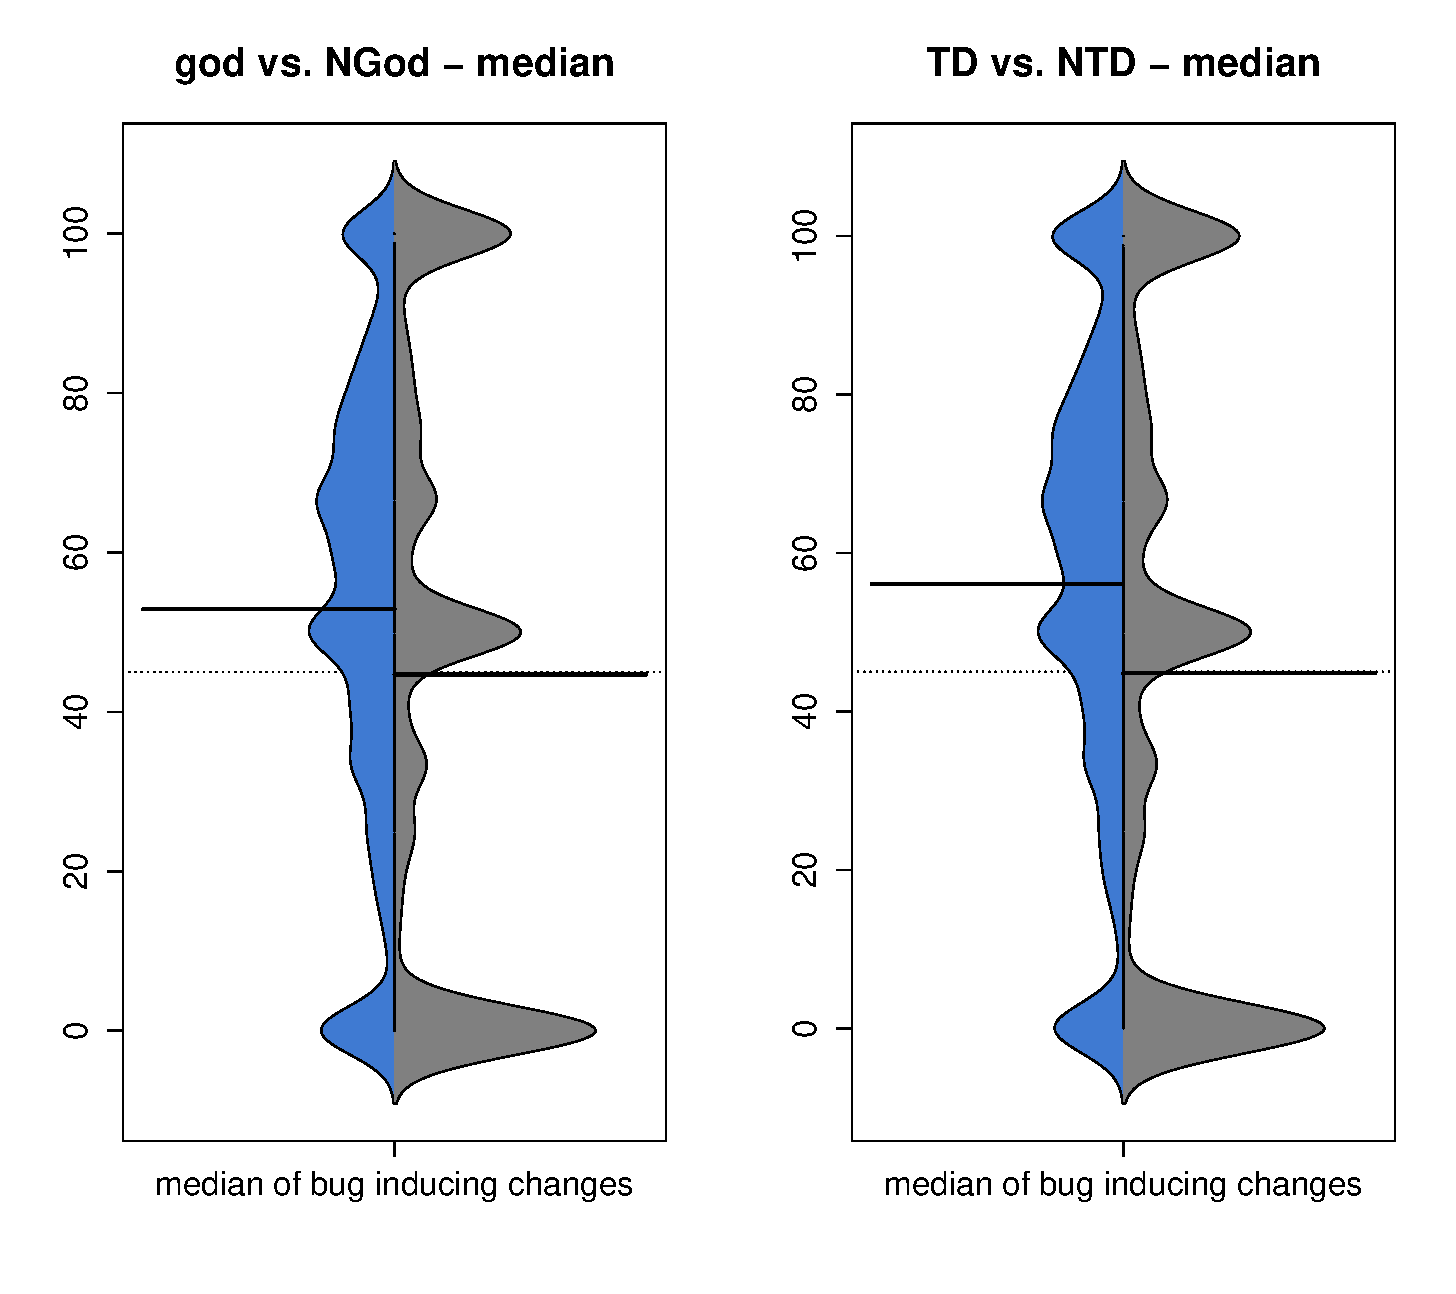
\includegraphics[width=140mm]{figures/chapter4/rq2_distrubtion_god_and_td}
	\caption{Percentage of defect inducing changes for (god vs. NGod) and (SATD and NSATD).}
	\label{figure:ch4_bug_inducing_changes}
\end{figure}

\subsection*{\chapterIVrqII}


\noindent{\textbf{Motivation:}}
Having looked at how god and non-god and SATD and non-SATD compare at the file level, we turn our sights to the question of whether the god and SATD changes introduce future defects at a higher rate than non-god and non-SATD changes. Before entire files were the objects of our analysis; now we require a more fine-grained analysis tailored to assess individual changes.


To investigate (i) how change category relates to introduction of future defects and (ii) the duration of the "grace period" before god and SATD changes impact software quality, we should begin by determining to what extent god classes and SATD are predisposed to introduce future defects. If a god or SATD change causes a defect to be introduced in the change right after, then the delay is minimal and the impact on quality cannot be put off for very long. Our conjecture is that god and SATD changes are more complex overall and introduce defects at a higher rate than non-god and non-SATD changes.


\noindent{\textbf{Approach:}}
We identify defect-inducing changes utilizing the SZZ algorithm~\cite{sliwerski-msr-2005} and subdivide the results it generates into four categories depending on whether the changes contain god classes or not (god vs. non-god defect-inducing changes) and SATD or not (SATD vs. non-SATD defect-inducing changes).\\ \\ \\


\noindent{\textbf{Results:}}

God change and non-god change distributions of defect-inducing change rates in each project share a common \textit{y}-axis in the first plot in Figure \ref{figure:ch4_bug_inducing_changes}, as do SATD change and non-SATD change defect-inducing change rate distributions in the second. For each plot, the distribution median (i.e. the median of the individual project medians) is higher for the variable-positive groups (god changes and SATD changes) than for variable-negative groups (non-god changes and non-SATD changes). This indicates that god and SATD changes have more of a tendency to induce future defects than their non-god and non-SATD counterparts.

As a general rule, what is true of the distribution medians is also true of individual project medians, though exceptions exist, among them Apache Hbase, Apache Kafka, Apache Mina, Apache Shiro, Apache Oozie, Apache Flink, Apache Deltaspike, Apache curator in Figures \ref{figure:percentage_of_bug_inducing_god_vs_ngod} and \ref{figure:percentage_of_bug_inducing_td_vs_ntd}, in which the variable-negative groups appeared to induce more future defects than the variable-positive groups. These isolated counterexamples, while in conflict with the trend observed in Figure \ref{figure:ch4_bug_inducing_changes}, are compatible with our findings in Chapter 3, where we report that SATD changes have less of a tendency to induce future defects.

\subsection*{\chapterIVrqIII}

\noindent{\textbf{Motivation:}}
Up to this point, we have been concentrating on the interplay between both god classes and SATD and defects lowering software quality. As we know from previous research \cite{marinescu2004detection}, god classes violate the object-oriented design principle and have negative long-term implications for system maintainability. Likewise, if we recall the ramifications of the technical debt metaphor, we see that the short-term payoff should come at an increased cost later on in development. The deferred consequences of god classes and technical debt are measured in terms of increasing difficulty, which has yet to be fully examined after detecting god classes and introducing technical debt.


Verifying that god classes and SATD do increase change difficulty will better portray their implications for future changes and software projects and in the end enable developers to see the full picture when deciding whether or not to refactor god classes or introduce \SATD. \\

\noindent{\textbf{Approach:}}
We recognize god, non-god, SATD and non-SATD change categories and compare the difficulty of effecting changes from each category. Four metrics are used to determine the change difficulty: churn (i.e. the total number of modified lines), the number of modified directories, the number of modified files, and the entropy of the change. For a slightly different purpose, Eick \emph{et al.}~\cite{eick2001decay} chose the first three to measure decay. As for the last metric, Hassan~\cite{hassan2009predicting} utilized it to measure change complexity.


To measure the change churn, number of files and number of directories, we extract these metrics from the change log. To calculate churn for a whole change, we add up the number of lines inserted and deleted in each individual file touched by the change. To count the files and directories touched by a change, we extract the list of files from the change log. We consider a directory to be \textbf{ND} and a file to be \textbf{NF} when measuring the number of modified directories and files. Thus, if a change involves the modification of a file having the path ``src/os/unix/ngx\_alloc.h``, then the directory is \textit{src/os/unix}, and the file is \textit{ngx\_alloc.h}.\\



\begin{figure}[tb!]
	\centering
	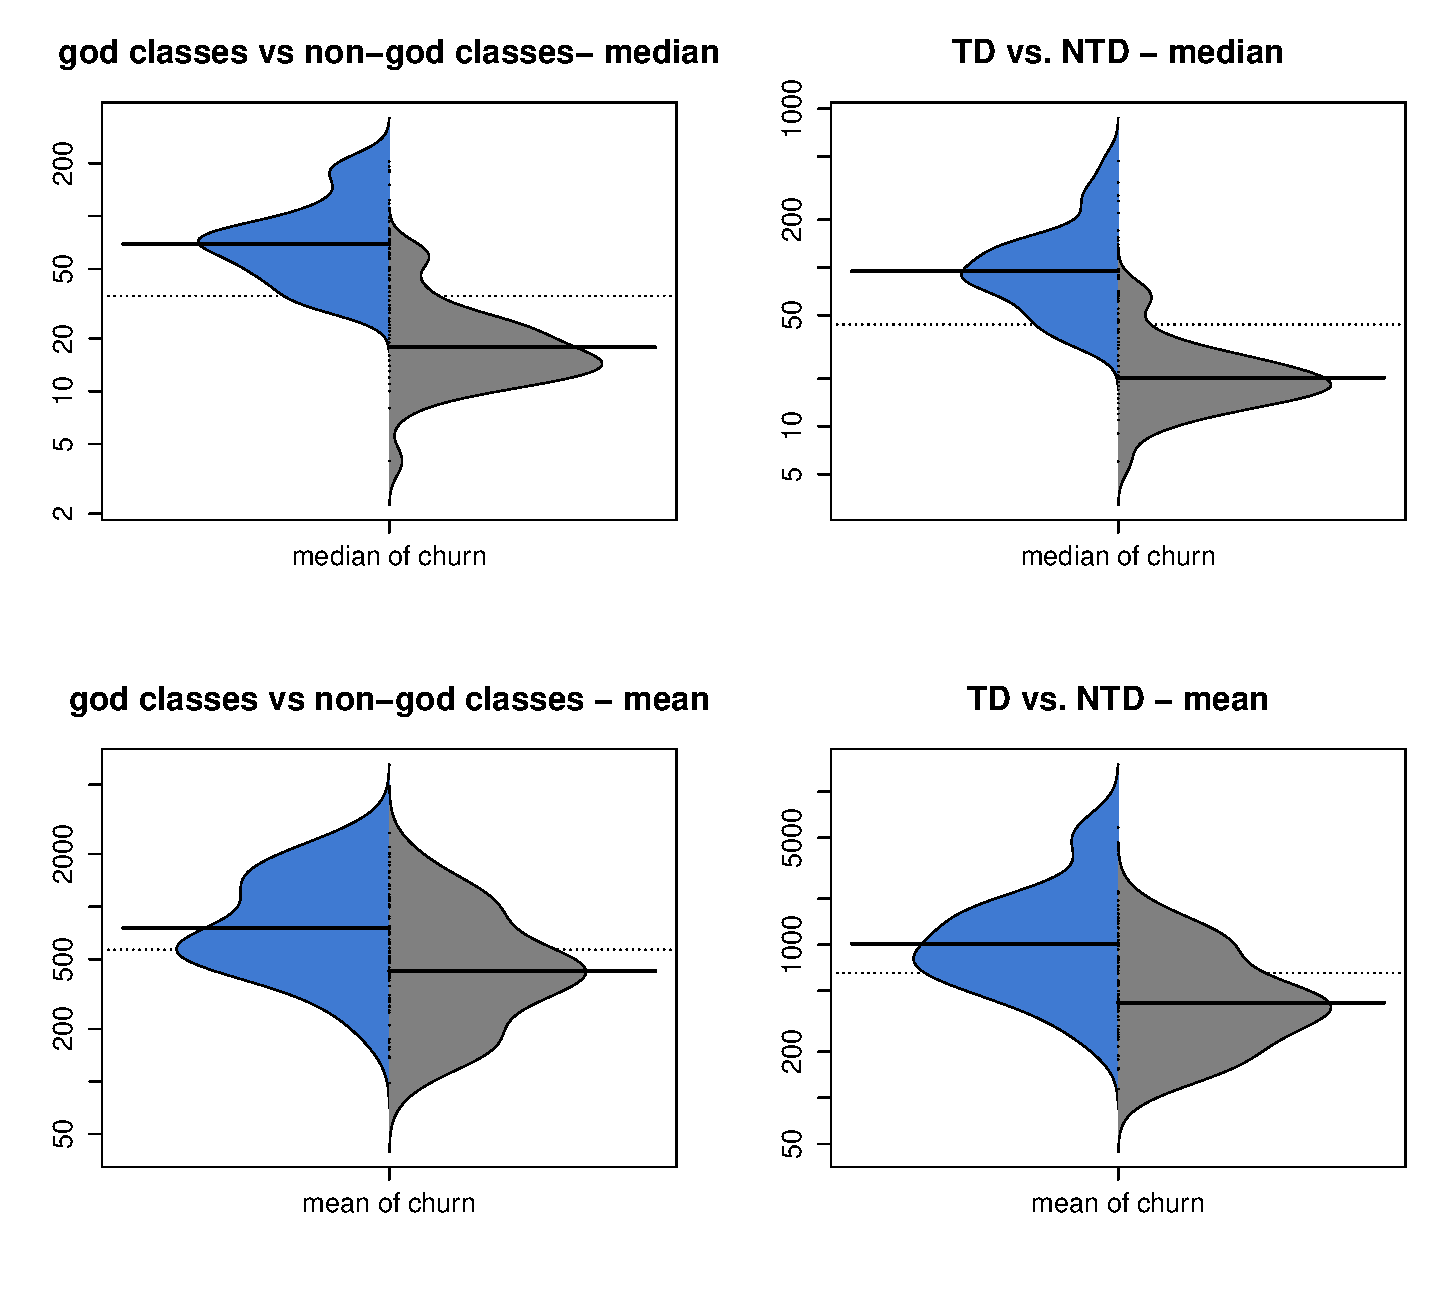
\includegraphics[width=120mm]{figures/chapter4/rq3_distribution_of_churn}
	\caption{Total number of lines modified per change (SATD vs. NSATD).}
	\label{figure:ch4_tlcpc}
\end{figure}



\begin{figure}[tb!]
	\centering
	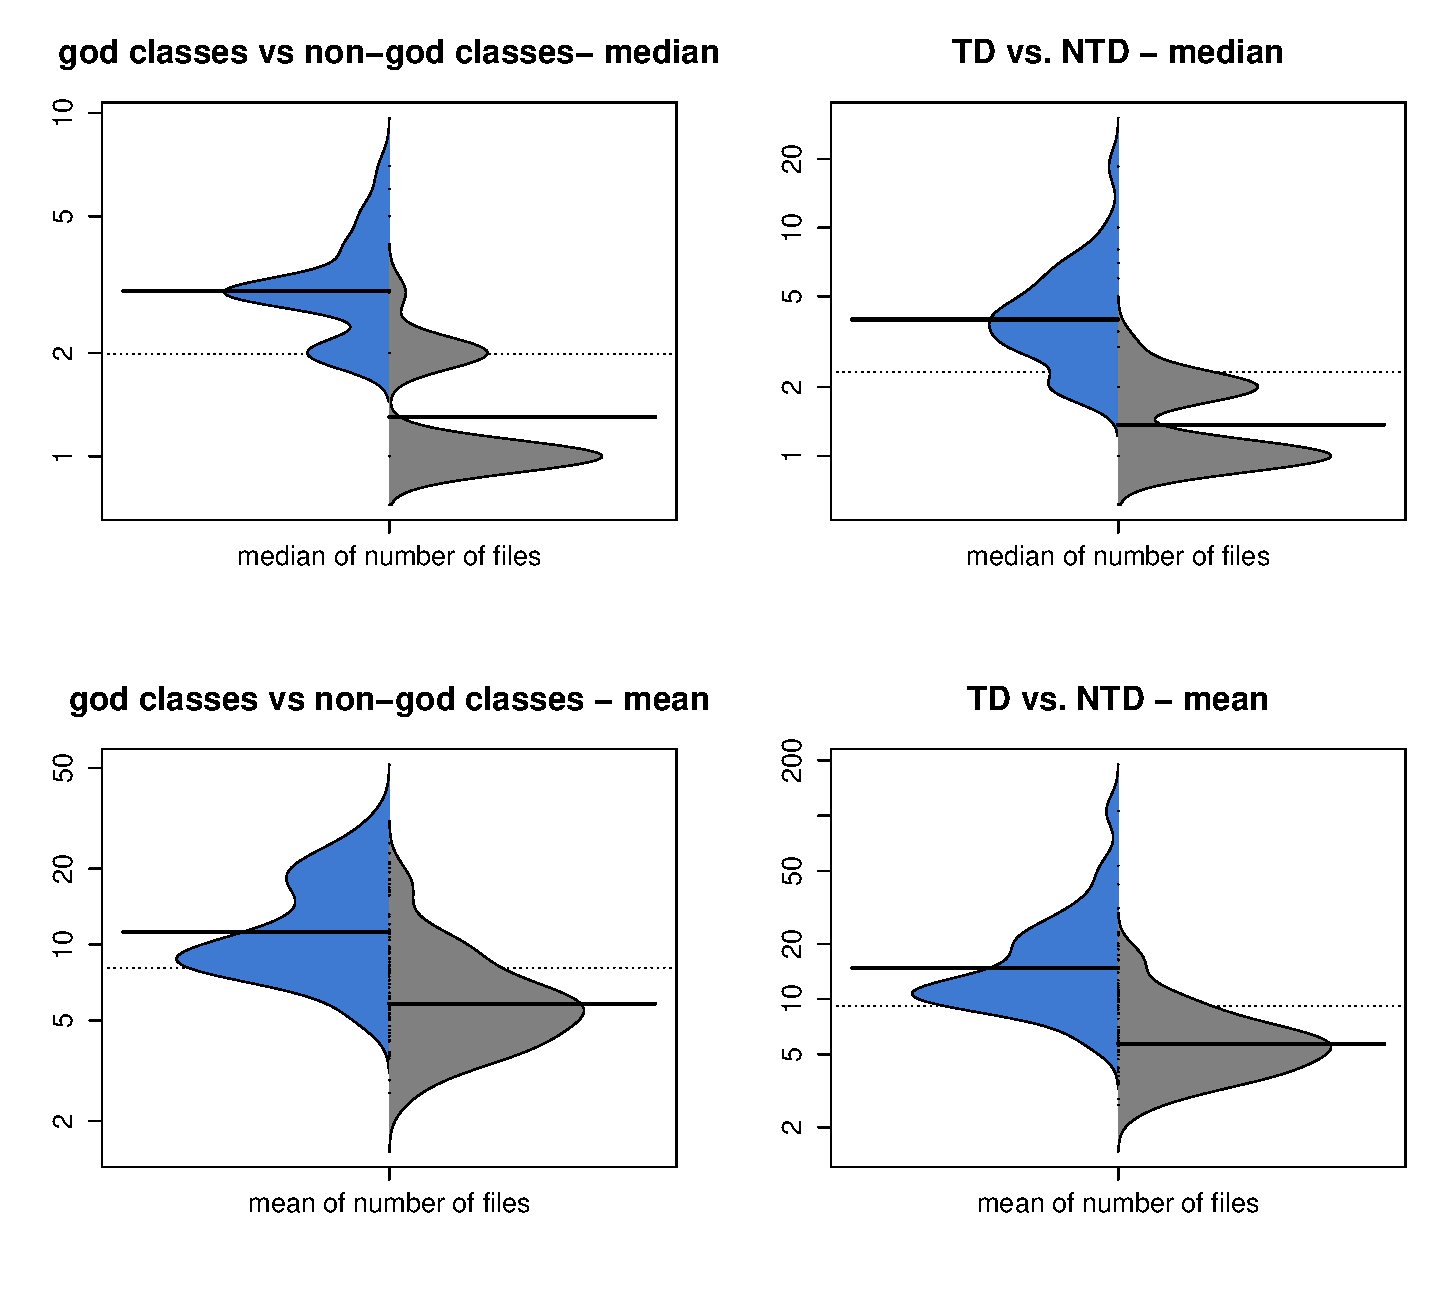
\includegraphics[width=120mm]{figures/chapter4/rq3_distribution_of_nf}
	\caption{Total number of files modified per change (SATD vs. NSATD).}
	\label{figure:ch4_tfcpc}
\end{figure}

\begin{figure}[!tb]
	\centering
	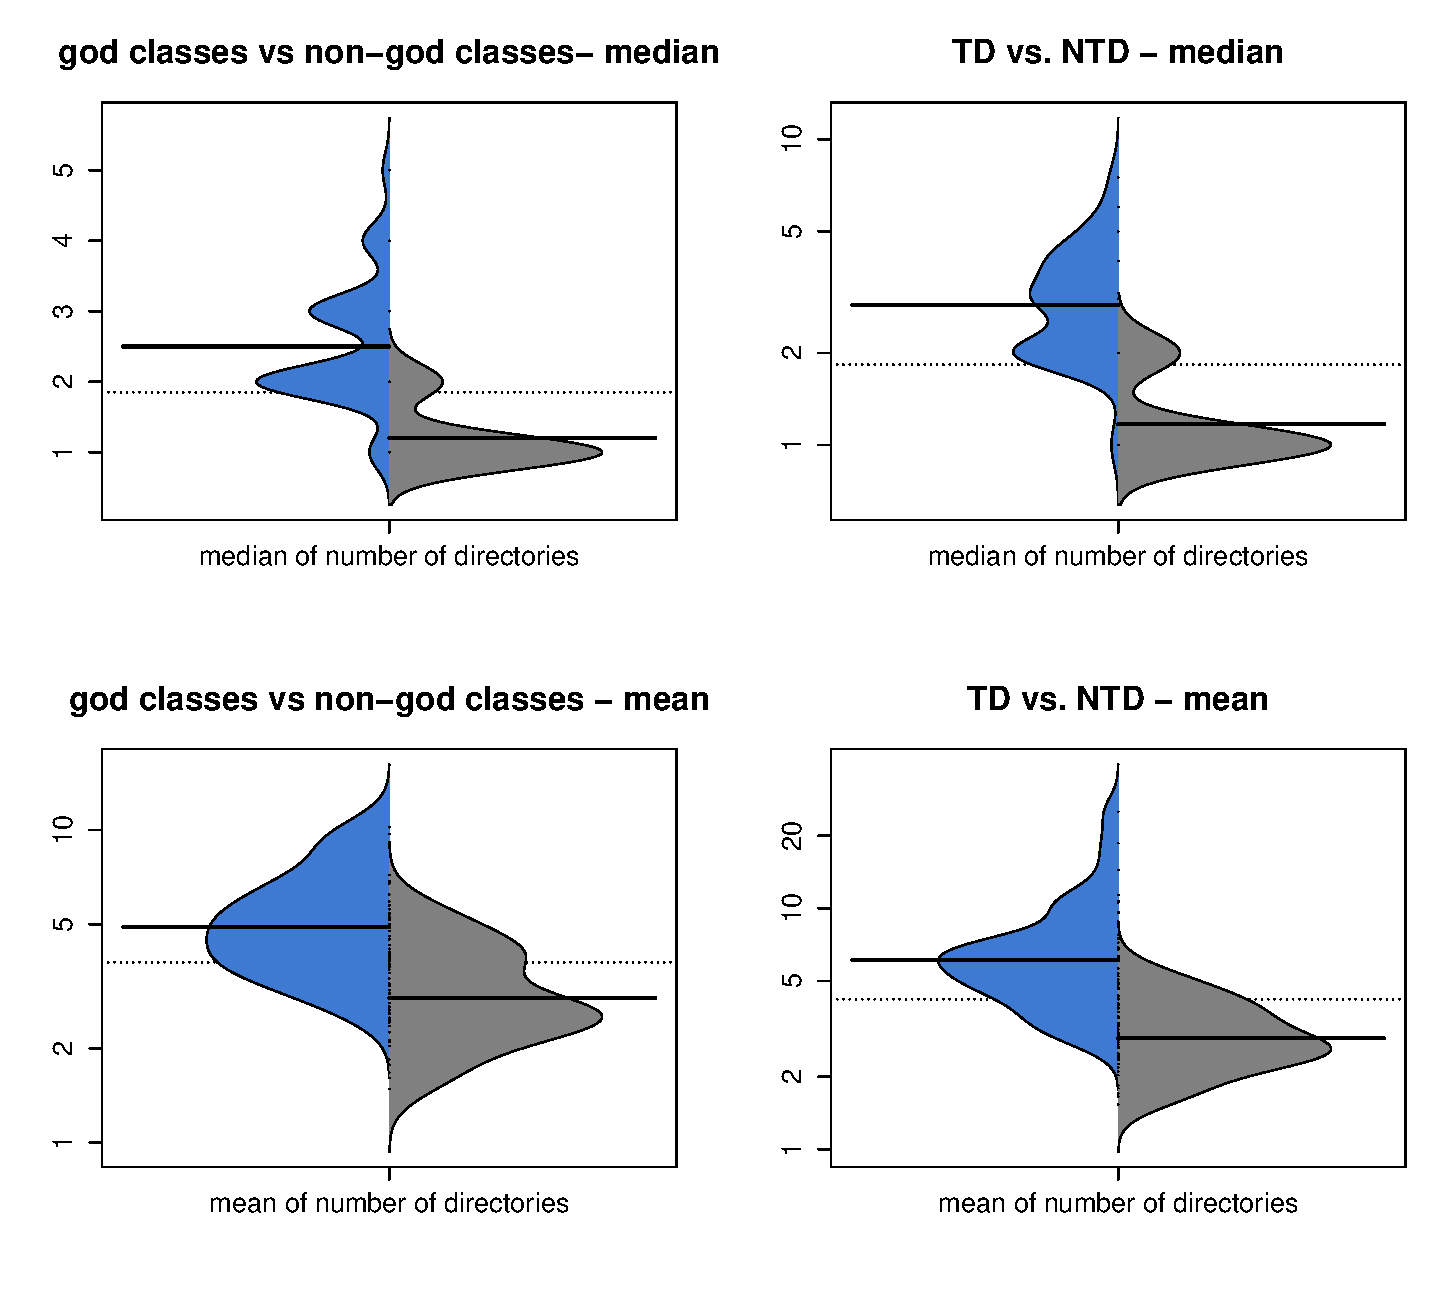
\includegraphics[width=120mm]{figures/chapter4/rq3_distribution_of_nd}
	\caption{Total number of modified directories per SATD and NSATD change.}
	\label{figure:ch4_umber_of_directories}
\end{figure}


\begin{figure}[!tb]
	\centering
	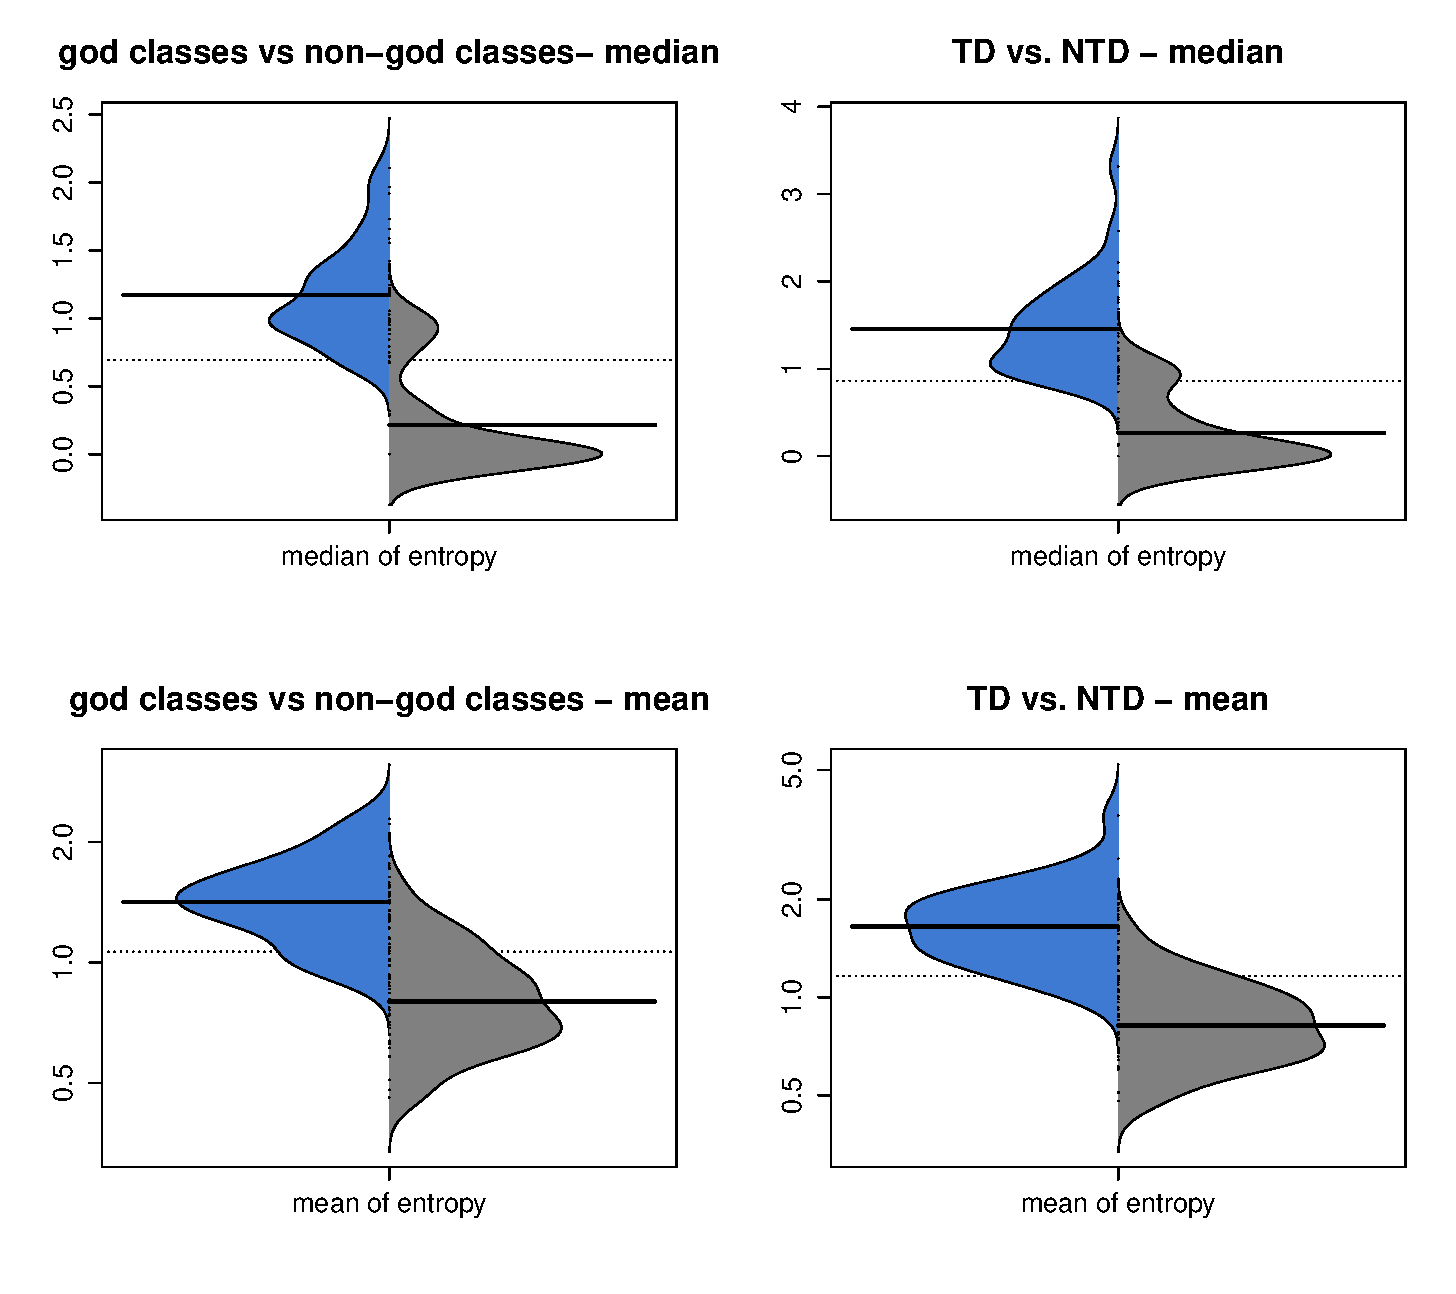
\includegraphics[width=120mm]{figures/chapter4/rq3_distribution_of_entropy}
	\caption{Distribution of the change across the SATD and NSATD files.}
	\label{figure:ch4_mtdocatdf}
\end{figure}



We adopt Hassan's change complexity measure~\cite{hassan2009predicting} to calculate change entropy, defined as $H(P)=-\sum _{k=1}^{n}\textrm ({p}_{k}*{log}_{2} {p}_{k})$, where $k$ is the proportion file$_{k}$ is modified in a change and $n$ is the number of files in the change. Entropy measures the distribution of a change across files. If we consider a change involving modification of three files \textit{A, B} and \textit{C}, for example, and take the number of lines modified to be 30, 1, and 1 lines respectively, the entropy equates to: $(0.40=-\frac{30}{32}\log_{2}\frac{30}{32}-\frac{1}{32}\log_{2}\frac{1}{32}-\frac{1}{32}\log_{2}\frac{1}{32})$.

The maximum entropy $log_{2}n$ has normalized the entropy formula presented above following Hassan~\cite{hassan2009predicting} so that entropy can be compared for changes touching different numbers of files. The higher the normalized entropy, the more difficult it is to make the change.\\

\noindent{\textbf{Results:}}


In each one of Figures~\ref{figure:ch4_tlcpc},~\ref{figure:ch4_tfcpc},~\ref{figure:ch4_number_of_directories},~\ref{figure:ch4_mtdocatdf}, a distribution is compiled for god and non-god and SATD and non-SATD changes by plotting the median values obtained from a different difficulty measure for each project. Juxtaposition of the \textit{distribution medians} demonstrates that regardless of the metric employed to quantify change difficulty (i.e. number of modified files, number of directories, amount of churn, or entropy), god and SATD changes are consistently more difficult to perform both on median and on mean than non-god and non-SATD changes.

Upon inspection of the boxplots in Figures~\ref{figure:total_number_of_lines_changed_god_vs_ngod},
~\ref{figure:total_number_of_lines_changed_td_vs_ntd},
~\ref{figure:total_nd_changed_god_vs_ngod},
~\ref{figure:total_nd_changed_td_vs_ntd},
~\ref{figure:total_files_god_vs_ngod},
~\ref{figure:total_files_td_vs_ntd},
~\ref{figure:total_entropy_god_vs_ngod},
~\ref{figure:total_entropy_td_vs_ntd}, we find that the distribution median and distribution mean inequalities remain unchanged for all projects for all difficulty measures except for OpenNLP for number of directories, where non-god and non-SATD change medians are still not greater than those of god and SATD changes but about equal.

In summary, we surmise that effecting god and SATD changes is more difficult than effecting non-god and non-SATD changes by all difficulty measures (i.e. number of modified files, number of directories, amount of churn, or entropy)




\subsection*{\chapterIVrqIV}

\todo{finish this research question}


\noindent{\textbf{Motivation:}}
Up to this point, we have compared the impact of technical debt identified by comment- and metric-based approaches on software quality. What remains outstanding now is the amount of overlap between the \SATD files that the comment-based approach labels and the god files that the metric-based approach detects. Specifically, our objective is to calculate the percentage of files that contain technical debt on both counts so that we can garner a better understanding of how comment-based technical debt complements metric-based technical debt.


\noindent{\textbf{Approach:}}
To address RQ4, we take the list of SATD files generated by the comment-based approach and the list of god files generated by the metric-based approach and isolate the files that made both lists. We count how many of these files meet the criteria for both approaches and then divide by the total number of files in both lists. The result represents the share of comment-based technical debt that complements the metric-based technical debt (overlap), expressed as a percentage.


\noindent{\textbf{Results:}}
Table~\ref{ch4_amount_of_overlap} displays the percentage overlap by project. We see that the values range from 11\% and 34\%. Our findings confirm that the comment-based approach, which uses source code comment patterns to detect technical debt, complements the metric-based approach, which relies on thresholds of object-oriented metrics. Despite the considerable overlap, each approach identifies some additional sources of technical debt that the other fails to detect.

	\begin{table}[htbp]
	\small
	\centering

		\begin{tabular}{l|c}
			\hline
			\textbf{Project}           & \textbf{Overlap (\%)} \\ \hline
			\textbf{Apache OpenNLP}    &    24.39     \\ \hline
			\textbf{Apache Camel}      &    16.57     \\ \hline
			\textbf{Apache Habse}      &    33.88     \\ \hline
			\textbf{Apache Groovy}     &    30.10     \\ \hline
			\textbf{Apache Oltu}       &    16.68     \\ \hline
			\textbf{Apache Maven}      &    26.08     \\ \hline
			\textbf{Apache Karaf}      &    23.65     \\ \hline
			\textbf{Apache Hama}       &    29.51     \\ \hline
			\textbf{Apache Tomee}      &    21.61     \\ \hline
			\textbf{Apache Deltaspike} &    20.46     \\ \hline
			\textbf{Apache Curator}    &    25.23     \\ \hline
			\textbf{Apache Calcite}    &    31.12     \\ \hline
			\textbf{Apache Poi}        &    31.36     \\ \hline
			\textbf{Apache Zeppelin}   &    23.37     \\ \hline
			\textbf{Apache Ant}        &    28.86     \\ \hline
			\textbf{Apache Stanbol}    &    32.95     \\ \hline
			\textbf{Apache Kafka}      &    20.64     \\ \hline
			\textbf{Apache Tika}       &    33.56     \\ \hline
			\textbf{Apache Felix}      &    26.00     \\ \hline
			\textbf{Apache Phoenix}    &    30.99     \\ \hline
		\end{tabular}
\quad \quad \quad
\begin{tabular}{l|c}
	\hline
			\textbf{Project}           & \textbf{Overlap (\%)} \\ \hline
			\textbf{Apache Wicket}     &    19.33     \\ \hline
			\textbf{Apache Aurora}     &    26.44     \\ \hline
			\textbf{Apache Ignite}     &    14.28     \\ \hline
			\textbf{Apache Helix}      &    25.45     \\ \hline
			\textbf{Apache Archiva}    &    30.33     \\ \hline
			\textbf{Apache Struts}     &    24.74     \\ \hline
			\textbf{Apache Derby}      &    32.56     \\ \hline
			\textbf{Apache Ambari}     &    25.59     \\ \hline
			\textbf{Apache Nifi}       &    18.92     \\ \hline
			\textbf{Apache Tiles}      &    11.37     \\ \hline
			\textbf{Apache Shiro}      &    31.03     \\ \hline
			\textbf{Apache Usergrid}   &    26.90     \\ \hline
			\textbf{Apache Nutch}      &    32.11     \\ \hline
			\textbf{Apache Zookeeper}  &    26.70     \\ \hline
			\textbf{Apache Mina}       &    16.78     \\ \hline
			\textbf{Apache Cxf}        &    22.25     \\ \hline
			\textbf{Apache CloudStack} &    27.91     \\ \hline
			\textbf{Apache Oozie}      &    21.88     \\ \hline
			\textbf{Apache Kylin}      &    22.54     \\ \hline
			\textbf{Apache Flink}      &    15.37     \\ \hline
\end{tabular}
	\caption{Percentage of overlap between god and SATD files of the analyzed projects.}
\end{table}



\section{Threats to Validity}
\label{chap4:sec:threats_to_validity}


Threats to \textbf{internal validity} concern any factors that could have confounded our study results. Since developers might not think to declare the introduction of a technical debt in the first place, or remove the corresponding comment after eliminating a technical debt, one candidate is the use of source code comments. Every time the code and comment do not undergo a change simultaneously, the source code comments become a less and less accurate record. Despite this, Potdar and Shihab~\cite{ICSM_PotdarS14} found that in Eclipse code and comments were updated in tandem 97\% of the time. Another threat derives from comments intended to indicate SATD that do not correspond to any of the patterns Potdar and Shihab~\cite{ICSM_PotdarS14} compiled, which, owing to the flexibility of natural language, had to be analyzed manually. This technique is error-prone and somewhat subjective, in that developers could conceivably disagree as to which comments indicate SATD consistently. To mitigate these effects, we conducted manual inspections of all identified comments for each project in turn to certify that each contained one of the 62 patterns in \cite{ICSM_PotdarS14}. While we chose to identify any change containing at least one SATD file as an SATD change, we could have reserved this label for changes containing only SATD files. In our view, it is better not to restrict SATD changes in this way because sometimes all it takes is one SATD file to change several other files touched by the same change.


Threats to \textbf{external validity} concern the generalizability of our results. In order to optimize this, we analyzed forty large open-source systems and drew our data from the well-established, mature codebase of open-source software projects with well-commented source code. Programming language and domain varied from project to project. Moreover, we focused on the relationship between SATD and god classes only, which means that other, unadmitted technical debt or code smells might have been overlooked. Nonetheless, studying all technical debt is beyond the scope of this thesis.

%We  believe the number of the analyzed systems  is sufficient enough to generalize our results. However,  we cannot be sure  that our findings  will be valid for other domains, applications,  programming languages, or proprietary  projects.

%Furthermore, we focused on SATD and god classes relationship only, which means that we do not cover all technical debt and therefore there may be other technical debt that is not self-admitted or a code smell. Studying all technical debt is beyond the scope of this thesis.





\section{Conclusion}
\label{chap4:sec:conclusion}


The software development community stigmatizes technical debt, even though it still lacks adequate evidence to formalize its adverse effects on software quality. Accordingly, the empirical study we present in this chapter seeks to identify in what ways god classes and self-admitted technical debt detract from quality. God classes centralize the workload of trivial classes and perform tasks using their data in violation of the object-oriented design principle stipulating one task per class. Self-admitted technical debt encompasses bugs that develop over time as a result of resorting to quick fixes that ``do the job" for the deadline and defer associated costs which could jeopardize the code in the long run. We identify god classes by employing Marinescu's \cite{marinescu2004detection} object-oriented metric thresholds and SATD by locating source code comments that match the SATD indicator patterns in \cite{ICSM_PotdarS14}.


Three correlations allowed us to dissect the relationship between god classes and software quality: (i) whether god files have more defects than non-god files, (ii) whether god changes introduce future defects and (iii) whether god changes are more difficult to perform. Likewise, we examine the impact of \SATD on quality by determining (i) whether SATD files have more defects than non-SATD files, (ii) whether SATD changes introduce future defects and (iii) whether SATD-related changes are more difficult to perform. We measured change difficulty for both god classes and \SATD in terms of the amount of churn, numbers of files and modified modules in a change and entropy.


In the end, we found that (i) there is no dependable trend between god classes or \SATD and defects: three exceptional projects revealed more corrective changes in SATD files than in non-SATD files; (ii) a trend did surface, however, in that both god changes and SATD changes are more correlated with the introduction of future defects and (iii) more difficult to perform than non-god and non-SATD changes. 

Our study imparts that although god classes and technical debt may have detrimental effects, these imply nothing with respect to defects per se, but increase the number of defect-inducing changes and make the system more difficult to change in the future. 